\section{Date: 2026-09-10}
\noindent \textbf{Series ID: JTS2300QUR} 

\noindent This series is titled Quits: Construction and has a frequency of Monthly. The units are Rate and the seasonal adjustment is Seasonally Adjusted.The observation start date is 2000-12-01 and the observation end date is 2026-07-01.The popularity of this series is 13. \\ 

\noindent \textbf{Series ID: WFHCOVIDFRACMATWOMEN} 

\noindent This series is titled Work from Home Rate: Women and has a frequency of Monthly. The units are Percent of Full Paid Working Days and the seasonal adjustment is Not Seasonally Adjusted.The observation start date is 2020-05-01 and the observation end date is 2026-08-01.The popularity of this series is 6. \\ 

\subsection{Raw Regression}
\noindent Regresses the two series against each other directly. A significant result here can come just as easily from both series sharing a long-run trend as from any real relationship.

\begin{center}
\begin{tabular}{lclc}
\toprule
\textbf{Dep. Variable:}          & value\_fred\_WFHCOVIDFRACMATWOMEN & \textbf{  R-squared:         } &     0.000   \\
\textbf{Model:}                  &                OLS                & \textbf{  Adj. R-squared:    } &    -0.013   \\
\textbf{Method:}                 &           Least Squares           & \textbf{  F-statistic:       } &   0.03323   \\
\textbf{Date:}                   &          Thu, 10 Sep 2026         & \textbf{  Prob (F-statistic):} &    0.856    \\
\textbf{Time:}                   &              15:17:47             & \textbf{  Log-Likelihood:    } &   -240.33   \\
\textbf{No. Observations:}       &                   74              & \textbf{  AIC:               } &     484.7   \\
\textbf{Df Residuals:}           &                   72              & \textbf{  BIC:               } &     489.3   \\
\textbf{Df Model:}               &                    1              & \textbf{                     } &             \\
\textbf{Covariance Type:}        &             nonrobust             & \textbf{                     } &             \\
\bottomrule
\end{tabular}
\begin{tabular}{lcccccc}
                                 & \textbf{coef} & \textbf{std err} & \textbf{t} & \textbf{P$> |$t$|$} & \textbf{[0.025} & \textbf{0.975]}  \\
\midrule
\textbf{const}                   &      32.4960  &        3.704     &     8.774  &         0.000        &       25.113    &       39.879     \\
\textbf{value\_fred\_JTS2300QUR} &      -0.3289  &        1.804     &    -0.182  &         0.856        &       -3.926    &        3.268     \\
\bottomrule
\end{tabular}
\begin{tabular}{lclc}
\textbf{Omnibus:}       & 71.083 & \textbf{  Durbin-Watson:     } &    0.194  \\
\textbf{Prob(Omnibus):} &  0.000 & \textbf{  Jarque-Bera (JB):  } &  449.811  \\
\textbf{Skew:}          &  2.992 & \textbf{  Prob(JB):          } & 2.11e-98  \\
\textbf{Kurtosis:}      & 13.492 & \textbf{  Cond. No.          } &     12.7  \\
\bottomrule
\end{tabular}
%\caption{OLS Regression Results}
\end{center}

Notes: \newline
 [1] Standard Errors assume that the covariance matrix of the errors is correctly specified.

\begin{figure}
\centering
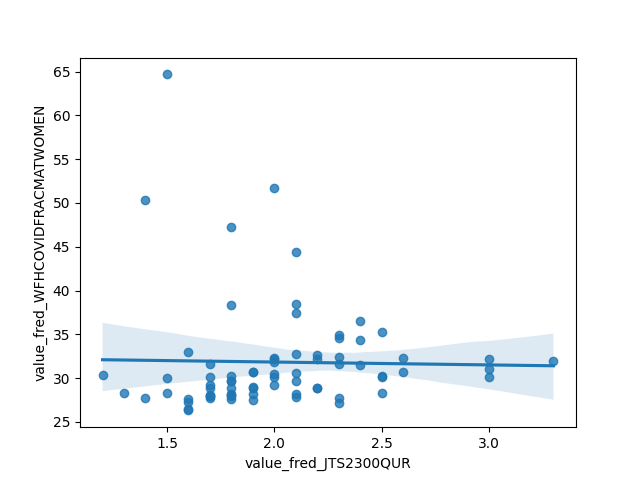
\includegraphics[scale = 0.9]{plots/plot_2026-09-10.png}
\caption{Raw Regression Plot for 2026-09-10}
\end{figure}
\newpage
\subsection{Detrended Regression}
\noindent Regresses the residuals of each series after removing its own linear time trend, so a shared trend can no longer drive the result on its own. A relationship that stays significant here is better evidence of a genuine link between the two series.

\begin{center}
\begin{tabular}{lclc}
\toprule
\textbf{Dep. Variable:}                     & value\_fred\_WFHCOVIDFRACMATWOMEN\_detrended & \textbf{  R-squared:         } &     0.300   \\
\textbf{Model:}                             &                     OLS                      & \textbf{  Adj. R-squared:    } &     0.290   \\
\textbf{Method:}                            &                Least Squares                 & \textbf{  F-statistic:       } &     30.84   \\
\textbf{Date:}                              &               Thu, 10 Sep 2026               & \textbf{  Prob (F-statistic):} &  4.44e-07   \\
\textbf{Time:}                              &                   15:17:47                   & \textbf{  Log-Likelihood:    } &   -205.78   \\
\textbf{No. Observations:}                  &                        74                    & \textbf{  AIC:               } &     415.6   \\
\textbf{Df Residuals:}                      &                        72                    & \textbf{  BIC:               } &     420.2   \\
\textbf{Df Model:}                          &                         1                    & \textbf{                     } &             \\
\textbf{Covariance Type:}                   &                  nonrobust                   & \textbf{                     } &             \\
\bottomrule
\end{tabular}
\begin{tabular}{lcccccc}
                                            & \textbf{coef} & \textbf{std err} & \textbf{t} & \textbf{P$> |$t$|$} & \textbf{[0.025} & \textbf{0.975]}  \\
\midrule
\textbf{const}                              &   -7.578e-12  &        0.460     & -1.65e-11  &         1.000        &       -0.917    &        0.917     \\
\textbf{value\_fred\_JTS2300QUR\_detrended} &      -7.2666  &        1.309     &    -5.553  &         0.000        &       -9.875    &       -4.658     \\
\bottomrule
\end{tabular}
\begin{tabular}{lclc}
\textbf{Omnibus:}       & 45.009 & \textbf{  Durbin-Watson:     } &    0.681  \\
\textbf{Prob(Omnibus):} &  0.000 & \textbf{  Jarque-Bera (JB):  } &  171.162  \\
\textbf{Skew:}          &  1.828 & \textbf{  Prob(JB):          } & 6.80e-38  \\
\textbf{Kurtosis:}      &  9.492 & \textbf{  Cond. No.          } &     2.84  \\
\bottomrule
\end{tabular}
%\caption{OLS Regression Results}
\end{center}

Notes: \newline
 [1] Standard Errors assume that the covariance matrix of the errors is correctly specified.

\begin{figure}
\centering
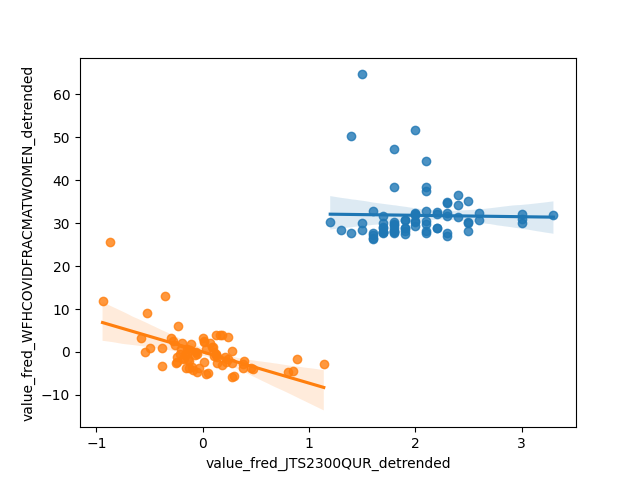
\includegraphics[scale = 0.9]{plots/plot_2026-09-10_detrended.png}
\caption{Detrended Regression Plot for 2026-09-10}
\end{figure}
\newpage
